\chapter{BACKGROUND}
\section{angr}
\citet{shoshitaishvili2016sok} described \code{angr} as “a binary analysis framework that integrates many of the state-of-the-art binary analysis techniques in the literature”. Within the framework are a multitude of static and dynamic analyses. Static techniques are those that derive meaning from a program without execution, while dynamic techniques derive meaning from an actual or emulated execution of the program \citep{shoshitaishvili2016sok}. Both paradigms of analyses are incredibly invaluable to the field of binary analysis as they each  provide unique insights into the structure, flow, and potential vulnerabilities of a binary. The proposed data dependency graph generation analysis is an example of a dynamic analysis, as it is reliant upon an ingested symbolic execution trace.
\section{Symbolic Execution}
As \citet{shoshitaishvili2016sok} discussed, symbolic execution is concerned with the emulation of a program. For the sake of data dependency, the fact that the emulation tracks the state of the register file and memory throughout the program’s lifetime is crucial, as it is used as the source of information for building out a data dependency graph \citep{shoshitaishvili2016sok}.

\begin{figure}
\begin{lstlisting}
0: endbr64
1: push   rbp
2: mov    rbp, rsp
3: mov    dword ptr [rbp-0x4], 0x1d6
4: mov    eax, dword ptr [rbp-0x4]
5: mov    dword ptr [rbp-0x8], eax
6: mov    eax, dword ptr [rbp-0x8]
7: pop    rbp
8: ret
\end{lstlisting}
\caption{Motivating example of data dependency}
\label{fig:motiv}
\end{figure}
\section{Data Dependency}
Data dependency maps the dependency relations between memory locations, in either the register file or within system memory, based on the data each location contains. Although, the memory location in question cannot be the sole consideration in determining a data dependency. As elucidated in the simple x86 code snippet (Figure \ref{fig:motiv}), it would be incorrect to treat the \code{eax} in the fourth and sixth instructions as the same data point when determining data dependencies. While their data regions are the same, both concerning the lower 32 bits of the \code{rax} register, they exist in different contexts during the program’s life cycle. Therefore, the point at which an instruction occurs must also be considered when determining which data points should be tracked. In this example, these memory locations can easily be differentiated by their instruction addresses.

With an understanding of the factors that must be considered in determining the data points established, the relationships between them can now be explored. A data point \emph{D$_1$} is considered dependent upon \emph{D$_2$} if the value of \emph{D$_1$} is derived from \emph{D$_2$}. Primarily, this derivation is the result of a read from  \emph{D$_2$} followed by a write of its value to \emph{D$_1$} (perhaps with some intermediary calculations). In the case of the motivating example (Figure \ref{fig:motiv}), the value of \code{[rbp - 0x8]} at instruction 5 is dependent upon the value of \code{eax} in instruction 5.

\begin{figure}
    \centering
    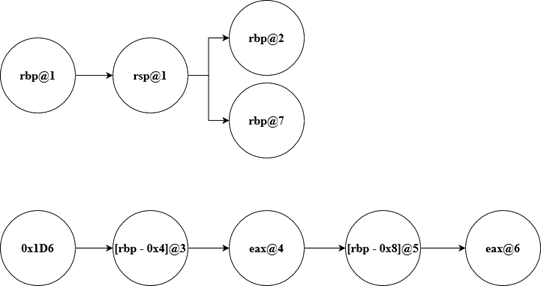
\includegraphics{ddg.png}
    \caption{DDG of motivating example, node names in form of location@address}
    \label{fig:motivddg}
\end{figure}

\section{Data Dependency Graph (DDG)}
A data dependency graph is a directed acyclic graph (DAG) that tracks all the data dependencies in a given execution trace. The data points, identified by their memory location and point of execution, serve as the graph’s nodes. The graph's edges originate from a source node and terminate at a dependent node. From any given node, one can follow the directed edges backwards to find the origin of a node’s value. By contrast, the edges leaving a node can be followed to find all dependent descendants in the data dependency graph. In the full dependency graph (Figure \ref{fig:motivddg}) of the code snippet provided in Figure \ref{fig:motiv}, the return value can be observed to have derived from a memory address ([rbp - 0x8]) which yielded its value from another address ([rbp - 0x4]) that had the constant written into it initially (with eax@4 being used to facilitate a memory to memory move in a RISC instruction set). While a toy example, it is evident that having a graphical representation of the flow of data within a more complicated program can prove invaluable to the binary analyst or software debugger.
\section{Intermediate Representation}
In compiler design, a source language can be translated into an arbitrary number of instruction sets. Thus, rather than developing optimizations for every unique target architecture, compilers utilize a middle-level, architecture-agnostic data structure instead. This data structure is referred to as the intermediate representation (IR). The source code is translated into IR before optimizations are applied and later converted into the target architecture instruction set. Just as compilers require an intermediary language to apply universal optimizations to source code, so too do decompilers such as \code{angr}’s. Although, in the case of decompilers, the process entails converting an arbitrary number of instruction sets back into a higher-level universal language. The intermediate representation used by \code{angr} is borrowed from Valgrind and is called VEX. Rather than operating on machine code, which would require a tremendous amount of architecture-aware code to handle the many cross-architecture idiosyncrasies, the proposed analysis operates on VEX IR.